
\chapter{Transverse Asymmetry} \label{transv}

\begin{itemize}

\item Physics behind the $A_{n}$ asymmetry, dependence on $Q^{2}$, the formula $\frac{\sigma_{\uparrow} - \sigma_{\downarrow}}{\sigma_{\uparrow} + \sigma_{\downarrow}}$
\item state of the art of the Exp.
\item Model description: so scattering amplitude, theoretical prediction
\item Expected error $ \delta A_{t} $
\item open question: problems with lead, dependence of $E_{beam}$, dependence from Z, Z/A
\end{itemize}

\section{Description of the process}

{\bfseries Explain the scattering process we are studying (at least one figure to visualize the kinematics of the scattering). Mention the link between this process and time-reversal operator. Add two figures for elastic and inelastic scattering.} 

The Beam Normal single spin asymmetry, which we will refer for brevity as Transverse asymmetry, originates from the interference of two scattering process. For the purpose of this thesis, we will present the case of electron scattering against a spin $0$ target \cite{Gorchtein_2008}.
To understand why the interference of this two scattering amplitude give rise to an asymmetry, we first have to look at the kinematic of the experiment: 

\begin{figure}[hbtp]
\centering
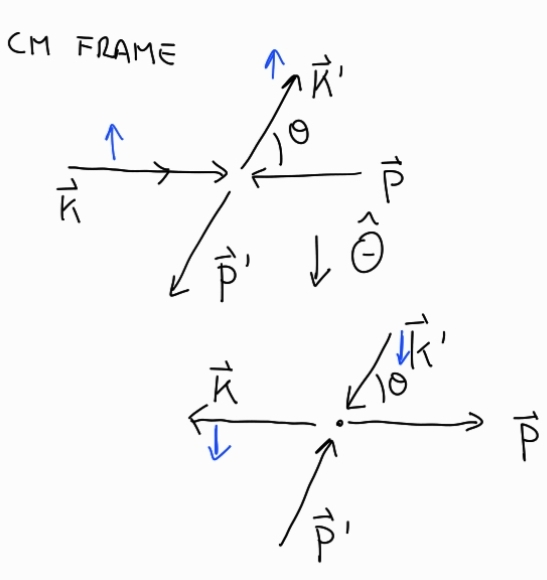
\includegraphics[width = 0.4\textwidth]{figures/Kinematic.jpg}
\caption{•}
\end{figure}

Where all the momenta are measured respect to the center of mass frame. In the figure we can confront the two situation before and after applying the Time-reversal operator, $\hat{\Theta}$. Looking at the picture we can understand that : 

\begin{itemize}
\item Before applying $\hat{\Theta}$, we have the incident electron with $\vec{k}$ momenta and the nucleus with $\vec{P}$ momenta, after applying $\hat{\Theta}$ we have that the incident/outgoing electron and the incident/outgoing nucleus are exchanged.
\item The $\hat{\Theta}$ operator acts also on the spin of the electron. Because we are considering process where the spin doesn't flip, the two situations are not equivalent.
\item Considering that the process is elastic, the kinematic is the same, taking $\vec{p}$ and $\vec{k}$ as the initial particle momenta, or $\vec{p}'$ and $\vec{k}'$. 

\end{itemize}

The time-reversal operator seems to connect the two different cases of UP and DOWN polarized electron. Our effort is to measure the asymmetry between the two cross section:

\begin{equation}
A = \frac{\sigma_{\uparrow} - \sigma_{\downarrow}}{\sigma_{\uparrow} + \sigma_{\downarrow}}
\end{equation}

And it's particularly clear that a non-zero asymmetry depends on how the time-reversal act on the elastic amplitude of the process. \\
With this idea, let's see in more detail the $\hat{\Theta}$. We know that $\hat{\Theta}$ is an antiunitary operator that can be always seen as:

\begin{align*}
\hat{\Theta} = U \cdot K
\end{align*} 
Where $U$ is an unitary operator, while $K$ is the complex conjugation operator that generates the complex conjugate of each coefficient in front of it. If we cosider a ket describing a system we have that:

\begin{equation}
Kc \ket{\alpha} = c^{*} K \ket{\alpha}
\end{equation}

Now, let's consider $H$ as the hamiltonian of our system. We want to apply the $\hat{\Theta}$ operator. We can now use the assumption that the hamiltonian consist of two term, which correspond to the two different scattering process. Because of the electromagnetic interaction conserve $CP$, so also $T$ is conserved, we know in advance that each piece of the hamiltonian commute with $\hat{\Theta}$. Now let's see what happen for an hamiltonian which has an imaginary part:

\begin{equation}
H = H_{R} + i H_{Im} \quad ; \quad \hat{\Theta} H \hat{\Theta}^{-1}= \hat{\Theta}H_{R} \hat{\Theta}^{-1} + \hat{\Theta} i H_{Im} \hat{\Theta}^{-1} \Rightarrow H_{R} - i H_{Im} \neq H
\end{equation}

what we understand from these simpe calculation is that to give rise to an asymmetry, we expect an imaginary part of the scattering amplitude different from zero.\\
At the $\alpha$ leading order, the two process of the electron-Nucleus scattering that give rise to the asymmetry involve the exchange of one-photon-exchange (OPE) and two-photon-exchange (TPE). The Feynman diagrams that describes the processes are the following: 

\begin{figure}
\[
\feynmandiagram [scale = 1, transform shape][baseline = (h), horizontal = d to j]{
	a [particle = \(e^{-}\)] -- [fermion, thick] c -- [fermion, thick ] f -- [fermion, thick] g [particle = \(e^{-}\)],
	c -- [photon, edge label = \(\gamma\)] d [blob],
	f -- [photon, edge label = \(\gamma\)] j [blob],
	h [particle = \(C^{12}\)]-- d -- [fermion, thick] j -- k [particle = \(C^{12}\)] ,
	};
\qquad
\feynmandiagram [scale = 1, transform shape][ vertical = c to d]{
	a [particle = \(e^{-}\)] -- [fermion, thick] c -- [fermion, thick] g [particle = \(e^{-}\)],
	c -- [photon, edge label' = \(\gamma\), momentum = {[arrow style = red]\(k\)}] d [blob],
	h [particle = \(C^{12}\)] -- [fermion, thick] d -- [fermion, thick] j [particle = \(C^{12}\)],
	};
\]
\caption{TPE and OPE diagrams in electron nucleus scattering.}
\end{figure}


A seguire come si scrive l'ampiezza per il termine elastico ed inelastico, aggiungere in appendice come viene fatto l'integrale sullo spazio delle fasi e stop. 



\subsection{Elastic scattering}

{ \bfseries Write the amplitude for the elastic (how to manipulate expression, maybe in the appendix). }



\subsection{Inelastic scattering}

Explain how it's possible to compute the inelastic expression, what kind of approximations are used (optical theorem...) 

\subsection{Model description}
Present the theoretical formula for the Transverse asymmetry, and comment on energy, Z, Z/A depencencies \\

adding together the elastic and inelastic contributions, we end with the following formula which describes the process \cite{PhysRevLett.121.022503}:

\begin{equation}
A_{N} = C_{0} \cdot log(\dfrac{Q^{2}}{m_{e}^{2} c^{2}}) \dfrac{F_{Compton}(Q^{2})}{F_{ch}(Q^{2})}
\end{equation}

\section{State of the Experiment}

Write down the formula $\frac{\sigma_{\uparrow} - \sigma_{\downarrow}}{\sigma_{\uparrow} + \sigma_{\downarrow}}$. Hints at how to measure the Transverse asymmetry (remember to mention we have a polarized beam against a unpolarized target). Explain the expected error for the recostructed asymmetry. Furthemore talk about the last mesurements obtained by the other collaborations, an outlook of the current situation. Maybe add also how we proceed to measure the transverse asymmetry, so the structure of the event, polarities patterns...
\bigskip

We have seen so far how the Transverse Asymmetry is related to the interference between two scattering amplitude, and the theoretical model used to describe the process. The goal from an experimental point of view is to measure this quantity. The challenge is to obtain a valid measure of $A_{n}$, which is of the order of $20$ part per million (ppm), taking into consideration all the possible effects that can interfere. To measure $A_{n}$, the straighfoward method is to prepare an electron beam, with polarized electron, and send it to a fixed target. The scattered electrons are then collected by a detector placed at a certain angle, and now it's possible to obtain the trasverse asymmetry applying the formula:

\begin{equation}
A_{} (Q,p) = \dfrac{N_{\uparrow}(Q) - N_{\downarrow}(Q)}{N_{\uparrow}(Q) + N_{\downarrow}(Q)} \cdot (\frac{1}{p})   
\end{equation} 

where we have explained the dependence on the transmitted impulse, on the degree of polarization of the beam.
In an experiment of this type, several requests are necessary to have an effective data acquisition:

\begin{itemize}
\item The accelerator must produce a polarized beam, stable over the time, with an high polarization percentage, in order to amplify the effect.
\item The Beam energy needs to be quite stable, and should not depend on the Polarization state of the electrons. A change in the Beam energy associated with the polarization state, can lead to a different count rate for $N_{\uparrow}$ and $N_{\downarrow}$, would make a contribution that would be added to that of the physical process
\item The beam must be correctly alligned with the target, and stable. Again if the position of the target changes accordin to the polarization of the electrons, it will produce another contribution to the total asymmetry.
\item The beam current should not depend on the polarization state of the electrons. If the beam source depends on the polarization, we will have a difference in the event rate and then another false asymmetry.
\item it's necessary to reject possible double elastic scattering events, which may contribute to the total asymmetry. 
\end{itemize}

All this demands can be satisfied with an accelerator that has stabilization devices with great precision and that can sustain high beam intensities. This last request is necessary to accumulate enough statistics to measure the transvere asymmetry with an accuracy about 1 ppm, in view of the future PV experiments. We can quantify how the statistical error varies according to the amount of data avaible. With the quite general assumption that the measured rate $N_{\uparrow,\downarrow}$ are gaussian distributed variables, we can compute the expected variance of $A_{n}$:

\begin{equation}
Var[A_{n}] = \dfrac{1 - A^{2}}{N_{\uparrow} + N_{\downarrow}} 
\end{equation}

This is the variance associated to a single measurement of the transverse asymmetry. As is well known, the variance scales as $\frac{1}{n}$ as $n$, the number of measures, increases.
Beacause the $A_{n}$ is expected to be quite small, we can approximate the above formula:
\begin{align*} \label{eq:SymmetryError}
V[A_{n}] = \dfrac{1}{2N \cdot n}
\end{align*}

The error associated to the recostructed asymmetry is the square root of the above quantity. If we impose that the error must be $\le 1ppm$ we can easily obtain that the quantity $n\cdot N$:

\begin{align*}
n\cdot N \le \frac{1}{2} \cdot 10^{12}
\end{align*} 

We will see later that achievable rates $N_{\uparrow,\downarrow}$ are in the range (20000,100000) for a carbon target. This number can not be increased at will by acting on the beam current. The first reason is obivios: the accelator and the beam source can handle only a certain amount of electrons before loosing their characteristics, furthermore a beam with great intensity for an extended periods of time can damage the carbon target, up to the risk of melting it. 
Another idea might be to increase the thickness of the target, to take advantage of the larger cross section. However this does not take into account that by doing so the number of double scattering event is increased. To avoid this the scientific community that deals with these nuclear physics measurements respect the convenction that the target thikness should be less than the $10 \%$ of the radiation lenght of the material.
